Архитектура кодировщик-декодировщик широко распространена в машинном обучении, теории кодирования, компрессии и
криптографии. В моделировании нейросетей также используют этот подход для задач \begin{itemize}
    \item генерации перевода и пересказа;
    \item классификации текста;
    \item распознания частей речи и выделения имен собственных.
\end{itemize}

\begin{figure}[h]
    \centering
    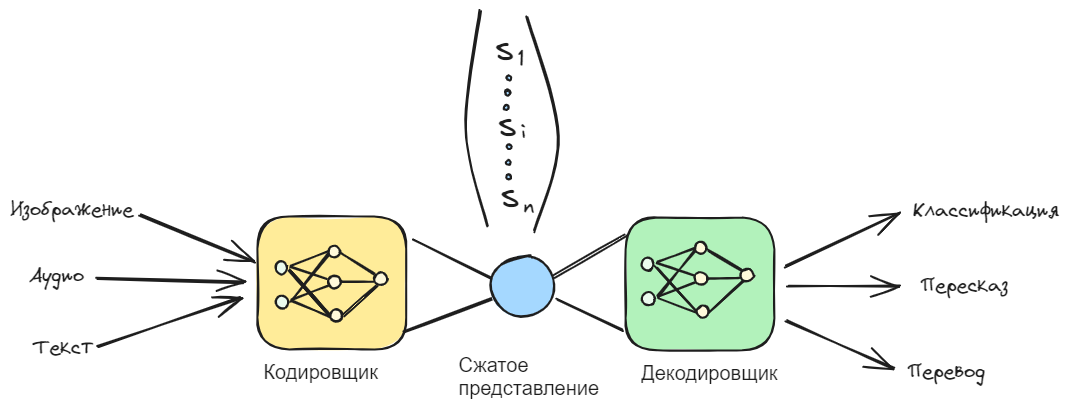
\includegraphics[width=0.5\textwidth]{assets/ml/nn/encoder_decoder.excalidraw.png}
    \caption{Преобразование сигнала выполняется в промежуточных слоях активации в ходе прямого распространения сигнала}
    \label{encoder}
\end{figure}

Такая архитектура 

\textit{Определение} Рекуррентными нейронными сетями называют такие, в которых используются скрытые состояния 
предыдущих слоев для расчета следующих.
\begin{equation}
    \begin{aligned}
        & h_t = \sigma (W_x x_t + W_h h_{t-1}+ b_h) \\
        & y_t = \sigma (W_y h_t + b_y), где \\
    \end{aligned}
\end{equation}
где \begin{itemize}
    \item $x_t$, $h_t$, $y_t$ векторы входного, скрытого и выходного слоя
    \item $W_x$, $W_h$, $W_y$ матрицы обновления состояния.
\end{itemize}
\begin{figure}[h]
    \centering
    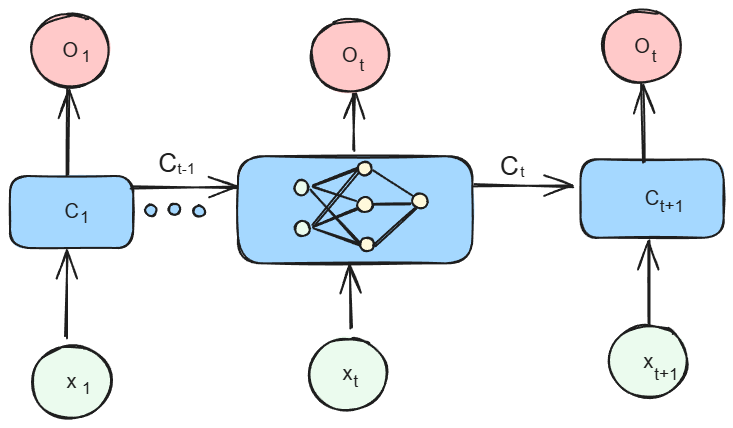
\includegraphics[width=0.5\textwidth]{assets/ml/nn/rnn.excalidraw.png}
    \caption{Каждая ячейка рекуррентной нейронной сети выполняет обновление представления.}
    \label{reccurent}
\end{figure}
Ошибка модели для случая обработки последовательностей равной длины запишется как:
\begin{equation}
    \mathcal{L}(\hat{y},y) = \sum_{t=1}^{T_y} \mathcal{L}(\hat{y},y)
\end{equation}
На практике матрицы обновления постоянны для каждой ячейки, поэтому правило обновления матрицы весов $W$ запишется как:
\begin{equation}
    \frac{\partial \mathcal{L}^{(T)}}{\partial W} = \sum_{t=1}^T \frac{\partial \mathcal{L}^{(T)} }{\partial W}
\end{equation}
Такой подход называется распространением ошибки во времени. Также существуют модификации механизма нейронной сети
заключающиеся в добавлении параллельного блока памяти \begin{itemize}
    \item долгая короткая память \cite{ochreiter1997long};
    \item управляемый рекуррентный блок \cite{chung2014empirical}.
\end{itemize}

Механизм внимания, основанный на модели рабочей памяти \cite{wallace1960plans}, позволил значительно улучшить результаты
задач перевода, пересказа и "понимания" языка \cite{bahdanau2014neural}.
Механизм внимания вычисляет вектор внимания \( \alpha \), который определяет важность каждого элемента входной 
последовательности на текущем временном шаге \cite{bahdanau2014neural}:
\begin{equation}
    \alpha_t = \text{softmax}(f(h_t, X))
\end{equation}
где \( f \) - функция, которая определяет важность каждого элемента входной последовательности, 
а \( \text{softmax} \) применяется для расчета нормированных весов внимания.

\begin{figure}[h]
    \centering
    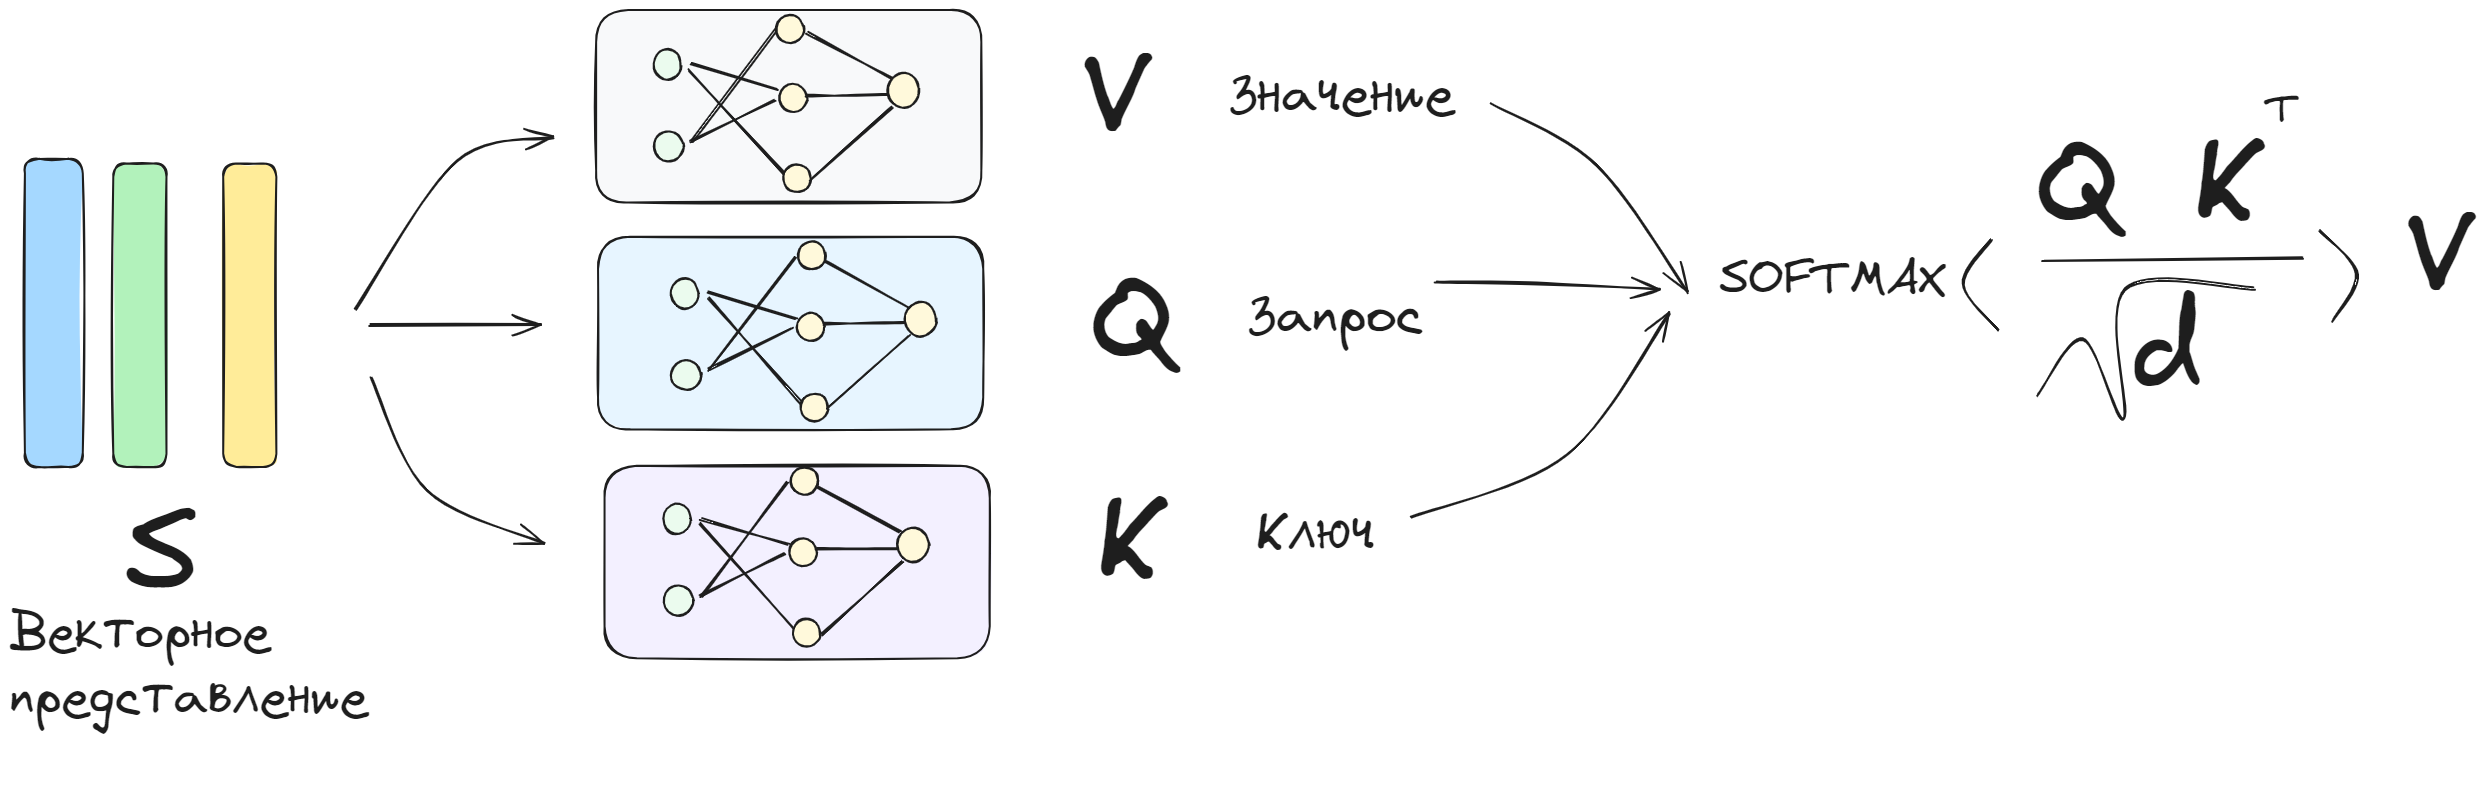
\includegraphics[width=0.5\textwidth]{assets/ml/nn/attention.excalidraw.png}
    \caption{Механизм внимания в архитектуре Transformer (Self Attention) \cite{vaswani2017attention} }
    \label{self_attention}
\end{figure}

Механизм внимания позволяет модели сосредоточиться на наиболее значимых частях входных данных в каждый момент времени, 
что делает его наиболее эффективным для задач, требующих адаптивности и контекстного понимания, таких как машинный перевод, 
генерация текста и вопросно-ответные системы. Этот механизм стал ключевым инструментом в области генеративного 
моделирования естественного языка, позволяя моделям эффективно работать с различными типами данных и контекстами.

